\documentclass[xcolor=dvipsnames,table]{beamer}

\usepackage{latexsym}
\usepackage[utf8]{inputenc}
\usepackage[brazil]{babel}
\usepackage{amssymb}
\usepackage{amsmath}
\usepackage{stmaryrd}
\usepackage{fancybox}
\usepackage{datetime}
\usepackage[T1]{fontenc}
\usepackage{graphicx}
\usepackage{graphics}
\usepackage{url}
\usepackage{algorithmic}
\usepackage{algorithm}
\usepackage{acronym}
\usepackage{array}

\newtheorem{definicao}{Definio}
\newcommand{\tab}{\hspace*{2em}}

\mode<presentation>
{
  \definecolor{colortexto}{RGB}{0,0,0}
 
  \setbeamertemplate{background canvas}[vertical shading][ bottom=white!10,top=white!10]
  \setbeamercolor{normal text}{fg=colortexto} 

  \usetheme{Warsaw}
}

\title{Grafos Conexos e Componentes} 

\author{
  Esdras Lins Bispo Jr. \\ \url{bispojr@ufg.br}
  } 
 \institute{
  Teoria de Grafos \\Bacharelado em Ciência da Computação}
\date{\textbf{04 de julho de 2017} }

\logo{
\includegraphics[width=1cm]{images/ufgJataiLogo.png}}

\begin{document}

	\begin{frame}
		\titlepage
	\end{frame}

	\AtBeginSection{
		\begin{frame}{Sumário}%[allowframebreaks]{Sumário}
    		\tableofcontents[currentsection]
    		%\tableofcontents[currentsection, hideothersubsections]
		\end{frame}
	}

	\begin{frame}{Plano de Aula}
		\tableofcontents
		%\tableofcontents[hideallsubsections]
	\end{frame}
    
   \begin{frame}{Pensamento}
   	\begin{columns}
   		\column{.4\textwidth}  		
   		\begin{center}
   			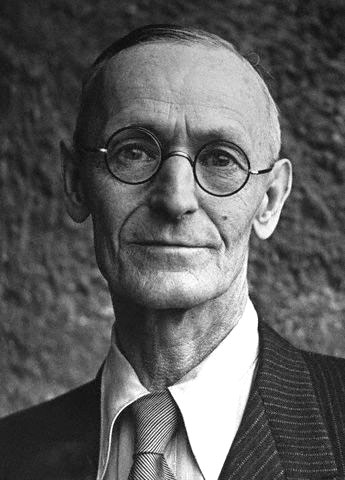
\includegraphics[width=.9\textwidth]{images/hesse.jpg}
   		\end{center}
   		\column{.6\textwidth}  		
   		\begin{block}{Frase}
   			\begin{center}
   				{\large Se você odeia alguém, é porque odeia alguma coisa nele que faz parte de você. O que não faz parte de nós não nos perturba.}
   			\end{center}
   		\end{block}		  		
   		\begin{block}{Quem?}
   			\begin{center}
   				{\bf Hermann Hesse (1877 - 1962)} \\Escritor e Pintor alemão.
   			\end{center}
   		\end{block}
   	\end{columns}
   \end{frame}
    
    \section{Revisão}
	\subsection{Subgrafos (cont.)}
	\begin{frame}{Subgrafos}
		\begin{block}{Subgrafo induzido - $G[X]$}
			O subgrafo de $G$ {\bf induzido} por um subconjunto $X$ de $V_G$ é \\o grafo $(X, F)$ em que $F$ é o conjunto $E_G \cap X^{(2)}$. \\Esse subgrafo é denotado por $G[X]$.
		\end{block}  
		\begin{block}{$G - X$}
			Para qualquer subconjunto $X$ de $V_G$, \\denotaremos por $G - X$ o subgrafo $G[V_G \setminus X]$.
		\end{block}  
		\begin{block}{$G - v$}
			Uma abreviação para $G - \{ v \}$.
		\end{block}
	\end{frame}
	
	\begin{frame}{Subgrafos}
		\begin{block}{$G - a$}
			Uma abreviação para o grafo $(V_G, E_G \setminus \{ a \})$.
		\end{block}  
		\begin{block}{$G - A$}
			Se $A$ é um subconjunto de $E_G$, então $G - A$ é uma abreviação para o grafo $(V_G, E_G \setminus A)$.
		\end{block}  
		\begin{block}{Corolário}
			$G - A$ é um grafo gerador de $G$.
		\end{block}
	\end{frame}

	\subsection{Caminhos e circuitos em grafos}
	\begin{frame}{Caminhos e circuitos em grafos}
		\begin{block}{Caminho em um grafo}
			Se um caminho $v_1 \ldots v_p$ é subgrafo de $G$, dizemos simplesmente que $v_1 \ldots v_p$ {\bf é um} caminho em $G$ ou que \\$G$ {\bf contém} o caminho $v_1 \ldots v_p$.
		\end{block}  
		\begin{exampleblock}{Circuitos em um grafo}
			Aplica-se identicamente a circuitos.
		\end{exampleblock} 
	\end{frame}
	
	\begin{frame}{Caminhos e circuitos em grafos}
		\begin{block}{Nomenclatura}
			Se $v$ e $w$ são os dois extremos de um caminho em $G$, é cômodo dizer que o caminho vai de $v$ a $w$ ou que começa em $v$ e termina em $w$.
		\end{block}  
		\begin{alertblock}{Cuidado!}
			Use estas expressões com cautela pois caminhos são objetos estáticos e não têm orientação.
		\end{alertblock}
	\end{frame}
	
	\begin{frame}{Caminhos e circuitos em grafos}
		\begin{block}{Caminho máximo em $G$}
			Um caminho $P$ em um grafo $G$ é máximo se $G$ não contém um caminho de comprimento maior que o de $P$.
		\end{block}  
		\begin{block}{Caminho maximal em $G$}
			Um caminho $P$ em $G$ é maximal se não existe caminho $P'$ em $G$ tal que $P \subset P'$.
		\end{block}  
		\begin{block}{Caminho Hamiltoniano}
			Um caminho é {\bf hamiltoniano} se contém todos os vértices do grafo.
		\end{block}
	\end{frame}	

	\section{Grafos Conexos e Componentes}
	\begin{frame}{Grafos Conexos}
		\begin{block}{Definição}
			Um grafo é {\bf conexo} se, para qualquer par $\{v,w\}$ de seus vértices, existe um caminho com extremos $v$ e $w$.
		\end{block} \pause
		\begin{block}{Subgrafo conexo maximal}
			Um subgrafo conexo $H$ de um grafo $G$ é maximal se $H$ não é subgrafo próprio de algum subgrafo conexo de $G$.
		\end{block} \pause
		\begin{block}{Componente}
			Um {\bf componente} (ou {\bf componente conexo}) de um grafo $G$ é qualquer subgrafo conexo maximal de $G$.
		\end{block}
	\end{frame}
	
	\begin{frame}{Grafos Conexos}
		\begin{block}{Corolário 1}
			Cada vértice de um grafo pertence a um e um só componente.
		\end{block} \pause
		\begin{block}{Corolário 2}
			Um grafo é conexo se e somente se tem um único componente.
		\end{block}
	\end{frame}
	
	\begin{frame}
		\titlepage
	\end{frame}
	
\end{document}